\documentclass{article}

% Language setting
% Replace `english' with e.g. `spanish' to change the document language
\usepackage[english,russian]{babel}
\usepackage{amsmath}

%графика
\usepackage{wrapfig}
\usepackage{graphicx}
\usepackage{pgfplots}
\usepackage{tikz}


\usepackage{tcolorbox}

% Set page size and margins
% Replace `letterpaper' with `a4paper' for UK/EU standard size
\usepackage[letterpaper,top=2cm,bottom=2cm,left=3cm,right=3cm,marginparwidth=1.75cm]{geometry}

% Useful packages
\usepackage{amsmath}
\usepackage{amssymb}
\usepackage{graphicx}
\usepackage{fixltx2e}
\usepackage[colorlinks=true, allcolors=blue]{hyperref}
\usepackage{caption} %заголовки плавающих объектов
\captionsetup[figure]{name=Рисунок}

\usepackage{geometry}
\geometry{left=25mm,right=25mm,
 top=25mm,bottom=25mm}

\title{Quantitative Analytics.\\
Lectures. Weeks 1-2. \\
Options Markets.\\
Рынки опционов.}
\author{Шарифуллин Александр}

% Колонтитулы
\usepackage{fancyhdr}
\pagestyle{fancy}
\renewcommand{\headrulewidth}{0.1mm}  
\renewcommand{\footrulewidth}{0.1mm}
\lfoot{}
\rfoot{\thepage}
\cfoot{}
\rhead{CMF-2022}
\chead{}

\begin{document}
\maketitle

% Оглавление
\setcounter{tocdepth}{1} % {2} - в оглавлении участвуют chapter, section и subsection. {1} - только chapter и section
\renewcommand\contentsname{Содержание}
\tableofcontents
\newpage

% \section{Dictionary, Definitions, Abbreviations}

% \subsection{Dictionary}
% \begin{itemize}
%     \item IR - Interest rate - процентная ставка.
%     \item Compounding - платежи (idk)
% \end{itemize}

% \subsection{Definitions and Abbreviations}
% \begin{itemize}
%     \item SAR - Stated annual rate.
%     \item EAR - Effective annual rate.
%     \item FoC - Frequency of Compounding
%     \item PMT - Payment
%     \item r - Interest rate (at the moment). 
% \end{itemize}

\renewcommand{\labelitemi}{\tiny$\bullet$}
\renewcommand{\figurename}{Fig.}

 \section{Понятие опциона}
 \subsection{Определение опциона}
 \textbf{Option (рус. -- опцион)} -- производный финансовый инструмент (дериватив), в котором сделка по покупке/продаже базового актива происходит только при определённых условиях.\\
 Покупатель опциона получает право на покупку/продажу некоторого базового актива по предопределённой цене в будущем. Право покупать или продавать базовый актив зависит от типа опциона. У продавца опциона в свою очередь может возникнуть обязательство по покупке/продаже базового актива по предопределённой цене в будущем. Это обязательство корреспондируется с правом покупателя опциона.\\
 Опцион имеет асимметричную структуру выплаты, то есть размеры выигрыша и проигрыша несимметричны. Опцион представляет собой игру с нулевой суммой -- выигрыш одной стороны несёт потери для другой.
\subsection{Типы опционов}
\begin{itemize}
    \item по типу заключаемой сделки:
    \begin{itemize}
        \item \textbf{опцион Call} -- опцион, дающий право его держателю купить в будущем базовый актив по предопределённой цене (называемой \textbf{страйком (strike price)}) у стороны, которая продала этот опцион;
        \item \textbf{опцион Put} -- опцион, дающий право его держателю продать в будущем базовый актив по предопределённой цене стороне, которая продала этот опцион;
    \end{itemize}
    \item по площадке совершения сделки:
    \begin{itemize}
        \item биржевые -- опционы, сделки о покупке/продаже которых совершаются на бирже;
        \item внебиржевые -- опционы, сделки о покупке/продаже которых совершаются на площадках, отличных от биржы;
    \end{itemize}
    \item по способу проведения сделки:
    \begin{itemize}
        \item поставочные -- опционы, при совершении сделок в рамках которых происходит поставка товара от продавца к покупателю;
        \item рассчётные -- опционы, при которых производится стоимостной расчёт прибыли/убытков покупателя и продавца без непосредственной поставки на основе текущий цены в момент совершения сделки;
    \end{itemize}
    \item по времени экспирации:
    \begin{itemize}
        \item европейский -- опцион, дающий право своему держателю покупать/продавать базовый актив в заисимости от типа опциона строго в моменты времени экспирации \(t\)
        \item американский -- опцион, дающий право своему держателю покупать/продавать базовый актив в заисимости от типа опциона в любой момент времени \(t\) до экспирации
    \end{itemize}
\end{itemize}
\section{Примеры опционов, доходности}
Рассмотрим пример опциона -- европейский опцион call.\\
Выплата по опциону call не включает в себя премию -- это просто разница в текущей стоимости опциона и прописанной в контракте.\\
Выплата по опциону call вычисляется по формуле:
\[Call\,payoff \,C = max(0, S_m - X),\;\text{где:}\]\\
\begin{itemize}
    \item \(S_m\) -- спотовая цена в момент времени \(m\);
    \item \(X\) -- цена покупки контракта (страйк-цена).
\end{itemize}
\textit{Интерпретация}: если цена базового актива на текущий момент меньше страйк-цены, то нет смысла пользоваться опционом (дешевле купить по спотовой цене на рынке): доходность опциона составит ноль. Если цена базового актива на текущий момент больше страйк-цены, то можно воспользоваться делегируемым опционом правом покупки базового актива по страйк-цене и поставить его на рынок по спотовой, тем самым получив выгоду, равную разнице между текущей спотовой ценой и страйк-ценой.\\
Рассмотрим, как выглядят графики доходности позиций для опциона call (рис. \ref{pic1_long_call_price}-\ref{pic2_short_call_price}). Положим, что инвестор приобрёл опцион call по цене 5\$ (опционная премия) со страйк-ценой равной 100\$ и сроком экспирации или сроком жизни опциона (option life) равным 2 месяцам.\\
\begin{figure}[h]
    \centering{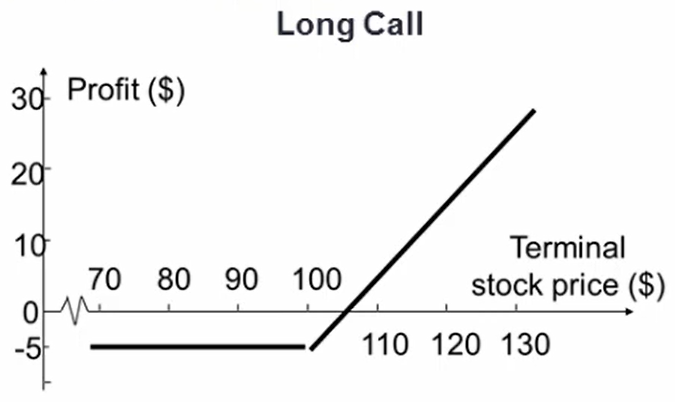
\includegraphics[width=0.4\textwidth]{pic1_long_call_price.png}}
    \caption{Зависимость доходность long-позиции от цены базового актива call-опциона}
    \label{pic1_long_call_price}
\end{figure}\\
\begin{figure}[h]
    \centering{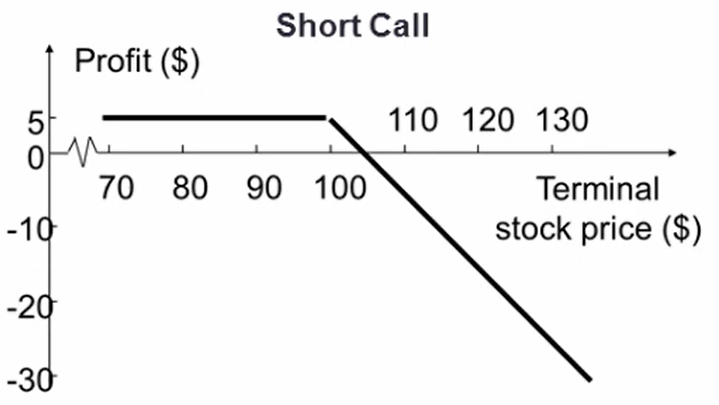
\includegraphics[width=0.4\textwidth]{pic2_short_call_price.png}}
    \caption{Зависимость доходность short-позиции от цены базового актива call-опциона}
    \label{pic2_short_call_price}
\end{figure}\\
Можно заметить, что представленные графики симметричны относительно оси абсцисс (стоковая цена (stock price) на момент закрытия опциона). Если сложим значения данных графиков, то получим позицию с нулевой суммой.\\
Начнём с длинной (long) позиции опциона call. До достижения стоковой цены значения 100\$ держатель опциона терпит убыток в размере 5\$, равный стоимости приобритения опциона. После превышения отметки в 100\$ убыток начинает падать, на отметке 105\$ достигается точка безубыточности (полностью покрываются расходы на уплаченную премию), а после данной точки при дальнейшем росте стоимости базового актива инвестор получает прибыль, при том неограниченную (чем выше цена, тем выше прибыль).\\
В случае с короткой (short) позицией опциона всё происходит симметрично -- продавший опцион получает премию в размере 5\$ и остаётся с данной прибылью до момента достижения стоимости базового актива отметки 100\$. После при дальнейшего росте цены доходность инвестора в short-позиции снижается, при отметке 105\$ становится равной нулю, после чего при последующем росте инвестор терпит убытки (при этом не ограниченные -- чем больше стоимость базового актива, тем больше убыточность short-позиции). \textit{Вывод}: продажа опциона call сопровождается значительными рисками, неограниченными в случае негативного сценария.\\
Для опциона put ситуация противоположна. Выплата по нему вычисляется по формуле:
\[Put\,payoff \,C = max(0, X - S_m)\]\\
Доходность от put-опциона отражена на рис. \ref{pic3_long_put_price}-\ref{pic4_long_put_price}.\\
\begin{figure}[h]
    \centering{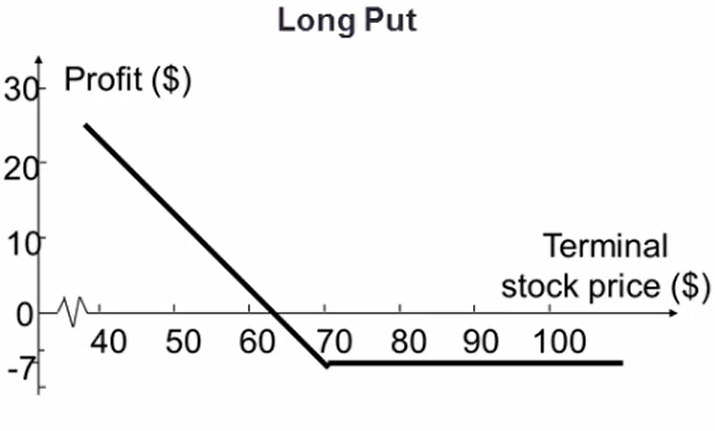
\includegraphics[width=0.4\textwidth]{pic3_long_put_price.png}}
    \caption{Зависимость доходность long-позиции от цены базового актива call-опциона}
    \label{pic3_long_put_price}
\end{figure}\\
\begin{figure}[h]
    \centering{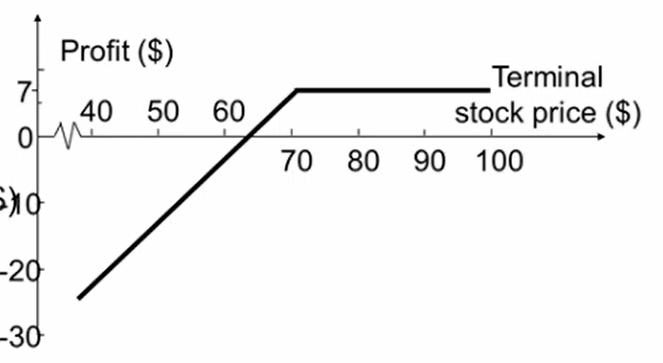
\includegraphics[width=0.4\textwidth]{pic4_long_put_price.png}}
    \caption{Зависимость доходность short-позиции от цены базового актива call-опциона}
    \label{pic4_long_put_price}
\end{figure}\\
Видим, что прибыль и убытки на этот раз ограничены нулевой стоимостью базового актива (в предположении о том, что цена не может быть отрицательной). В длинной позиции прибыль тем выше, чем меньше цена базового актива (в срок экспирации мы продаём базовый актив по страйк-цене, поэтому чем ниже спотовая цена, тем выше доходность). В короткой позиции прибыль тем выше, чем выше цена базового актива, но не больше, чем премия за опцион, а убыток тем больше, чем меньше цена за базовый актив  (при продаже опциона мы обязуемся при реализации держателем опциона права на продажу базового актива выкупить его по страйк-цене).\\
 \section{Базовые активы опционов}
 В качестве базовых активов может выступать практически что угодно. Биржевые опционы ограничены набором инструментов, торгуемых на бирже, внебиржевые -- ограничены договорённостями между сторонами опционного контракта.\\
 Распространённые опционы:
 \begin{itemize}
    \item опционы на \textbf{акции} (stock options) -- в качестве базового актива используются акции; 
    \item опционы на \textbf{валюту} (currency options) -- в качестве базового актива используются валютные пары;
    \item опционы на \textbf{индексы} (index options) -- в качестве базового актива используются индексы (чаще всего представлены европейскими расчётными опционами, могут быть как биржевыми, так и внебиржевыми);
    \item опционы на \textbf{фьючерсы} (futures options) -- в качестве базового актива используются фьючерсные контракты (могут быть только биржевыми, так как фьючерс по определению -- биржевой контракт);
\end{itemize}
\section{Концепция денежности опционов}
Существет классификация различных сценариев при экспирации опционного контракта, называемая денежностью опциона (moneyness). Денежность бывает:
 \begin{itemize}
    \item OTM (out of the money) -- ситуация для call/put опциона, при которой цена базового актива меньше/больше страйк-цены, таким образом опцион принесёт убыток инвестору; 
    \item ATM (at the money) -- ситуация для call/put опциона, при которой цена базового актива равна страйк-цене, таким образом опцион окажется безубыточным для инвестора;
    \item ITM (in the money) -- ситуация для call/put опциона, при которой цена базового актива больше/меньше страйк-ценs, таким образом опцион принесёт прибыль инвестору;
\end{itemize}
\textit{Примечание texer'а}: скорее всего, автор данной лекции подразумевал, что мы не учитываем опционную премию. В противном случае точка безубыточности равна не страйк-цене, а сумме страйк-цены и опционной премии.
\section{Компоненты цены опциона}
Цена опциона (option price) складывается из следующих компонент:
 \begin{itemize}
    \item внутренняя стоимость (intrinsic value) -- значение, равное возможному доходу держателя опциона, если бы времени до экспирации не оставалось и он экспирировался бы прямо сейчас;
    \item временная стоимость (time value) -- разница между опционной премией (option premium) и внутренней стоимостью.
\end{itemize}
\section{Классы и серии опционов}
Под \textbf{классом} опционов понимаются все опционы на один базовый актив.\\
Под \textbf{серией} опционов понимаются все опционы на один базовый актив и с одним сроком экспирации.\\
\section{Нестандартные опционные продукты}
Помимо классических опционов существуют нестандартные финансовые продукты, в основе которых также лежит идея в "опциональности" в зависимости от соотношения текущей спотовой и страйк-цен:
 \begin{itemize}
    \item \textbf{FLEX options} -- биржевые опционы, по которым можно изменить сменить спецификацию опциона (время до экспирации, страйк-цена, стиль -- call/put);
    \item \textbf{ETF (exchange trading funds) options} -- биржевые опционы (в основном американского типа), подразумевающие только поставки, а не расчёт;
    \item \textbf{Weekly options} -- биржевые опционы с малым сроком экспирации (short-term options), обычно формируемые в четверг и экспирируемые в пятницу следующей недели;
    \item \textbf{Binary options} -- краткосрочные опционы, фиксированные выплаты (обычно в размере процента от опционной премии) по которым производятся, когда цена касается значения выше (call-опцион) или ниже (put-опцион) страйк-цены, в противном случае инвестор терпит убыток в размере опционной премии;
    \item \textbf{CEB (credit event binary) options или CEBOs} -- совмещение кредитного события и бинарного опциона: выплата будет при наступлении кредитного события в размере некоторой фиксированной суммы;
    \item \textbf{DOOM options} -- структурированные как put-опционы, позволяют находиться иннвестору в состоянии ITM только при значительных просадках цены базового актива (страйк-цена таких опционов крайне мала); схожи с credit default swaps (выкуп кредитных обязательств в случае дефолта).
\end{itemize}
\section{Оценка эффекта от выплаты дивидендов и разделения акций}
 \begin{itemize}
    \item дивиденды (dividends) могут выплачиваться в денежном виде и виде других акций; в первом случае на спецификацию опциона никакого влияния не происходит (влияние только на оценку (pricing) опциона, во втором случае возникает ситуация, подобная сплиту, которая рассматривается ниже;
    \item при сплите (split) акций важно отношение акций \(a_before/a_after\), так как данное отношение как множитель меняет страйк-цену (если количество акций увеличилось вдвое, страйк-цена уменьшается также вдвое)
 \end{itemize}
\section{Термины опционной торговли (option trading)}
Важно понимать следующие термины, касающиеся опционной торговли:
 \begin{itemize}
    \item \textbf{маркетмейкеры или market makers} -- крупные участники, котирующие рынок, выставляющие твёрдые заявки (при запросе покупки маркетмейкер выставляет соответствующий bid, при запросе продажи -- соответствующий ask) на покупку/продажу в стакан/по запросу;
    \item \textbf{floor brokers} -- компании-посредники между публичными пользователями и рынком;
    \item \textbf{the order book official} -- сотрудники биржи, отвечающие за реализацию заявок от floor brokers;
    \item \textbf{an offsetting trade} -- противоположная сделка, закрывающая позицию;
    \item \textbf{открытый интерес или open interest} -- общее количество незакрытых контрактов.
 \end{itemize}
 \section{Комиссии, требования к маржинальной торговле}
 \textbf{Комиссии или commissions} состоят обычно из фиксированной части и доли от размера сделки.\\
 Опционы со сроком экспирации менее девяти месяцов не могут быть приобретены в рамках маржинальной торговли, так как кредитное плечо при таких сделках может оказаться слишком высоким (что ускорит обнуление депозита или наступление margin call).\\
 Обычно, кредит предоставляется не более чем в 25\% от стоимости опциона.
 \section{Упрощённая схема исполнения опционного контракта}
 Упрощённо, схему исполнения опционного контракта можно представить в виде следующией последовательности действий:
 \begin{itemize}
    \item инвестор принимает решение об исполнении опционного контракта;
    \item инвестор уведомляет брокера о намерении исполнить опционный контракт;
    \item брокер связывается с членом опциноной клиринговой корпорации (Options Clearing Corporation или OCC), ответственным за клиринг торговых операций данного брокера;
    \item данный член инициирует процедуру исполнения опционного контракта, находит противоположную сторону, продавшую опцион (соответственно взявшую на себя исполнить его обязательство);
    \item противоположная сторона обязуется продать/купить в зависимости от call/put опциона по страйк-цене базовый актив, сама операция должна происходить на третий рабочий день после получения ордера на исполнение;
    \item количество контрактов в обращении -- open-interest -- уменьшается на один;
    \item в случае, если держатель опциона не воспользовался своим правом, а опцион находится в состоянии ITM, вся выше перечисленная процедура будет инициирована брокером.
 \end{itemize}
 \section{Продукты, связанные с опционом на акцию}
Существует 4 основных продукта, связанные с опционами на акцию. Глобально эти четыре продукта можно разбить на два в зависимости от того, с кем осуществлён контракт -- с эмитентом этой акции или нет.\\
Опционный контракт, заключаемый с неэмитентом данной акции, не сопровождается размытием долей текущих инвесторов. Опционный контракт с эмитентом приводит к выпуску новых акций и сопровождается их размытием. Примеры размытия:\\
\begin{itemize}
    \item \textbf{конвертируемые облигации или convertible bonds} дают право держателю облигации обменять её на акцию по определённому conversion ratio, в этом случае эмитент обязуется погасить свои обязательства новыми выпускаемыми; акциями, что приводит к размытию доли;
    \item компенсация работникам с помощью опционов на акции компании -- эмитент в качестве мотивационного пакета выпускает опцион, реализуемый в виде акций, которые эмитент должен выпустить при экспирации опционов их держателями, что также приводит к размытию;
    \item \textbf{warrant} -- облигация+опцион, но при экспирации опциона облигация не исчезает, а при выпуске акций возможно размытие долей.
\end{itemize}


\end{document}
